% !TeX root = main.tex
\section{下载并安装 VSCode}
\begin{frame}[fragile]
  \frametitle{Windows 用户}
  \begin{itemize}[<+->]
    \item 在 VSCode 的官网 \href{https://code.visualstudio.com/}{https://code.visualstudio.com/} 选择 stable 版本进行下载
    \item 安装的时候注意将 ``通过 Code 打开'' 添加到上下文菜单:
  \end{itemize}
  \uncover<2>{
    \begin{center}
      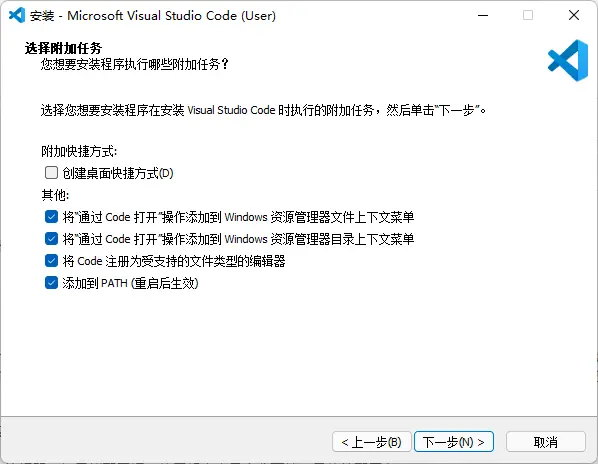
\includegraphics[width=8cm]{install-vs.png}
    \end{center}
  }
\end{frame}

\section{打开终端}

\begin{frame}[t]
  \frametitle{打开终端}
  \begin{description}[<+->]
    \item[WindowS 用户] 
    \begin{itemize}[<+->]
      \item \keys{\win + S} 后输入 ``cmd'' 并按下回车, 可以打开``命令提示符'', 也就是所谓的命令行, 或者使用 \keys{\ctrl + \shift + \enter} 来用管理员权限打开命令行.
      \only<2>{
        \begin{center}
          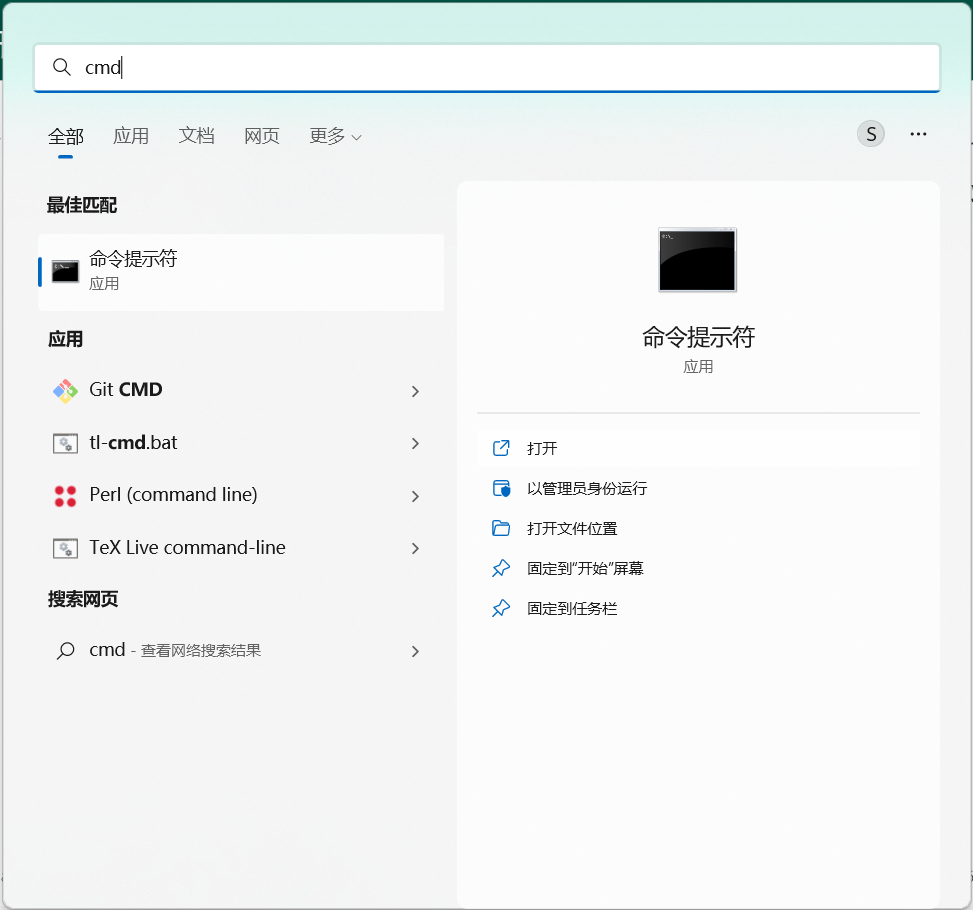
\includegraphics[width=6cm]{cmd.png}
        \end{center}
      }
      \item 在``文件资源管理器''的地址栏输入``cmd'' 并按下回车, 即可在当前位置打开命令行:
      \only<3>{
        \begin{center}
          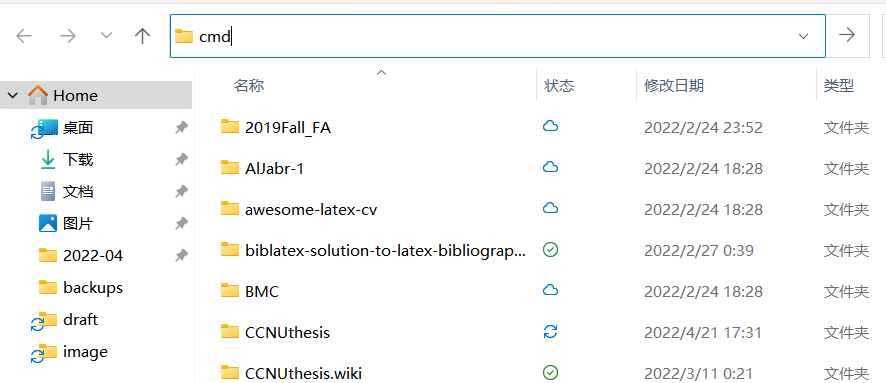
\includegraphics[width=7cm]{explorer.png}
        \end{center}
      }
      \item 如果安装了 Windows Terminal, 或者系统为 Win11, 可以在文件夹中或者文件夹上点击右键, 选择``在终端中打开'', 即可打开 Windows Terminal:
      \only<4>{
        \begin{center}
          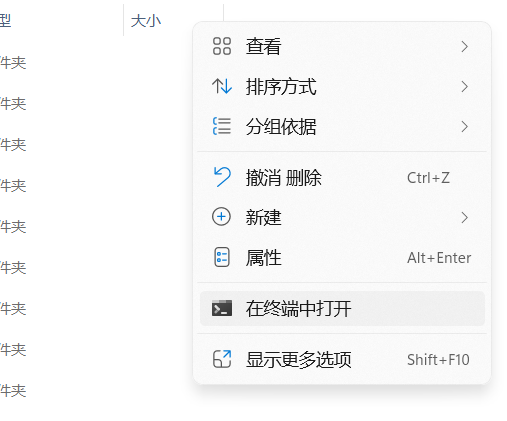
\includegraphics[width=5cm]{right-click.png}
        \end{center}
      }
    \end{itemize}
    \item[macOS 用户] \keys{\cmdmac + \SPACE} 后输入``terminal'', 即可打开终端. 
    \item[Linux 用户] \keys{\ctrl + \Alt + T} 即可打开终端. 
  \end{description}
  \uncover<7>{后面我们提到终端, 命令行均指这些东西, 并不做名字上的区分}
\end{frame}

\section{\tlmgr 的使用}
\subsection{\tlmgr 的简单介绍}
\begin{frame}[fragile]
  \frametitle{\tlmgr 的介绍}
  \begin{itemize}
    \item \tlmgr 是 \texlive 用来管理\emph{软件包}的工具;
    \item \emph{软件包}指的不只是可以通过 \lcmd{\usepackage} 调用的宏包, 而是所有 \texlive 包含的, 可以使用 \tlmgr 管理的内容, 比如平常所说的宏包, 如 \lstinline{amsmath.sty}, 一些说明文档, 如 \lstinline{lshort-zh-cn}, 一些可执行文件, 如 \lstinline{xetex.exe} 等等.
    \item \tlmgr 是 \textbf{T}eX\textbf{L}ive \textbf{M}ana\textbf{g}e\textbf{r} 的缩写;
    \item 命令行中运行 \cmd{tlmgr version} 就可以看到当前的\emph{修订版号}(revision), 通常输出如下
\begin{lstlisting}
tlmgr revision 63033 (2022-04-15 07:19:42 +0200)
tlmgr using installation: C:/texlive/2022
TeX Live (https://tug.org/texlive) version 2022
\end{lstlisting}
  \end{itemize}
\end{frame}

\subsection{\tlmgr 的基本语法}

\begin{frame}[fragile]
  \frametitle{\tlmgr 的基本语法}
\begin{cmdcode}
tlmgr --global-options action --action-specific-options operand
\end{cmdcode}
\begin{enumerate}
  \item \cmd{-} 与 \cmd{--} 相同;
  \item \cmd{-dry-run}.
\end{enumerate}
\end{frame}

\subsection{更新软件包}

\begin{frame}[fragile,t]
  \frametitle{更新软件包 --- 操作: \frameaction{update}}
  \framesubtitle<1>{查看哪些软件包可以更新}
  \begin{onlyenv}<1>
\begin{cmdcode}
tlmgr update -list
\end{cmdcode}
\begin{lstlisting}[basicstyle=\tiny\ttfamily,frame=single]<1>
tlmgr.pl: package repository https://mirrors.tuna.tsinghua.edu.cn/CTAN/systems/texlive/tlnet (not verified: gpg unavailable)
tlmgr.pl: would save backups to C:/texlive/2022/tlpkg/backups
tlmgr.pl: skipping forcibly removed package: collection-texworks
update:   adjmulticol   [316k]: local:  62935, source:  63073
update:   hitex         [2565k]: local:  62529, source:  63073
update:   texlive-fr    [1394k]: local:  62853, source:  63071
update:   texlive-msg-translations [144k]: local:  63010, source:  63072
update:   texlive-scripts.win32 [36k]: local:  62199, source:  63068
update:   texlive-scripts [504k]: local:  63049, source:  63068
update:   utfsym         [4766k]: local:  56729, source:  63076
update:   xduts          [871k]: local:  63013, source:  63075
update:   zwpagelayout   [641k]: local:  53965, source:  63074  
\end{lstlisting}
  \end{onlyenv}
  \framesubtitle<2>{更新全部软件包}
  \begin{onlyenv}<2>
\begin{cmdcode}
tlmgr update -self -all
\end{cmdcode}
\begin{lstlisting}[basicstyle=\tiny\ttfamily,frame=single]
tlmgr.pl: package repository https://mirrors.tuna.tsinghua.edu.cn/CTAN/systems/texlive/tlnet (not verified: gpg unavailable)
tlmgr.pl: saving backups to C:/texlive/2022/tlpkg/backups
tlmgr.pl: no self-updates for tlmgr available
[ 1/16, ??:??/??:??] update: babel-french [567k] (59997 -> 63088) ... done
[ 2/16, 00:02/01:48] update: l3backend [894k] (63025 -> 63089) ... done
...
[16/16, 01:23/01:23] update: collection-luatex [1k] (62829 -> 63081) ... done
running mktexlsr ...
done running mktexlsr.
running mtxrun --generate ...
done running mtxrun --generate.
running updmap-sys ...
...
tlmgr.pl: package log updated: C:/texlive/2022/texmf-var/web2c/tlmgr.log
tlmgr.pl: command log updated: C:/texlive/2022/texmf-var/web2c/tlmgr-commands.log
\end{lstlisting}
  \end{onlyenv}
  \framesubtitle<3>{其他的功能}
  \begin{enumerate}[<3->]
    \item 更新软件包 \pkg{pkg1}, \pkg{pkg2}:
\begin{cmdcode}
tlmgr update pkg1 pkg2
\end{cmdcode}
    \item 如果更新全部宏包时不想更新 \pkg{pkg1}, \pkg{pkg2}:
\begin{cmdcode}
tlmgr update -self -all -exclude pkg1 -exclude pkg2
\end{cmdcode}
    \item 如果更新过程被中断
\begin{cmdcode}
tlmgr update -self -all -reinstall-forcibly-removed
\end{cmdcode}
  \end{enumerate}
\end{frame}

\subsection{查看软件包信息}

\begin{frame}[fragile]
  \frametitle{查看软件包信息 --- 操作: \frameaction{info}}
  \framesubtitle<1>{列出软件包的详细信息}

  \begin{onlyenv}<1>
\begin{cmdcode}
tlmgr info pkg1 pkg2
\end{cmdcode}
\begin{lstlisting}[basicstyle=\tiny\ttfamily,frame=single]
package:     ctex
category:    Package
shortdesc:   LaTeX classes and packages for Chinese typesetting
longdesc:    ctex is a collection of macro packages and document classes for LaTeX Chinese typesetting.
installed:   Yes
revision:    61285
sizes:       src: 481k, doc: 1137k, run: 1753k
relocatable: No
cat-version: 2.5.8
cat-license: lppl1.3c
cat-topics:  chinese book-pub class
cat-contact-bugs: https://github.com/CTeX-org/ctex-kit/issues
cat-contact-support: https://github.com/CTeX-org/ctex-kit/issues
cat-contact-repository: https://github.com/CTeX-org/ctex-kit
cat-contact-home: http://www.ctex.org/HomePage
collection:  collection-langchinese
\end{lstlisting}
  \end{onlyenv}

  \framesubtitle<2>{查看软件包的文件信息}
  \begin{onlyenv}<2>
\begin{cmdcode}
tlmgr info -list pkg1 pkg2
\end{cmdcode}
\begin{lstlisting}[basicstyle=\tiny\ttfamily,frame=single]
# 省略 tlmgr info tabularray 的内容 #
Included files, by type:
run files:
texmf-dist/tex/latex/tabularray/tabularray-2021.sty
texmf-dist/tex/latex/tabularray/tabularray.sty
doc files:
texmf-dist/doc/latex/tabularray/README.txt details="Readme"
texmf-dist/doc/latex/tabularray/tabularray.pdf details="Package documentation"
texmf-dist/doc/latex/tabularray/tabularray.tex  
\end{lstlisting}
  \end{onlyenv}
\end{frame}

\subsection{回滚软件包的版本}

\begin{frame}[fragile]
  \frametitle{回滚软件包的版本 --- 操作: \frameaction{restore}}
  
  \framesubtitle<1>{查看某个软件包的备份} 
  % \begin{onlyenv}<1>
\begin{cmdcode}
tlmgr restore pkg
\end{cmdcode}
\begin{lstlisting}[basicstyle=\tiny\ttfamily, frame=single]
tlmgr restore functional
Available backups for functional: 62926 (2022-04-17 11:15)
\end{lstlisting}
  % \end{onlyenv}
  \framesubtitle<2>{将某个软件包回滚为备份}

\begin{uncoverenv}<2>
\begin{cmdcode}
tlmgr restore pkg revision
\end{cmdcode}
\begin{lstlisting}[basicstyle=\tiny\ttfamily, frame=single]
tlmgr restore functional 62926
Do you really want to restore functional to revision 62926 (y/N): y
Restoring functional, 62926 from C:/texlive/2022/tlpkg/backups/functional.r62926.tar.xz
running mktexlsr ...
done running mktexlsr.
running mtxrun --generate ...
done running mtxrun --generate.
tlmgr.pl: package log updated: C:/texlive/2022/texmf-var/web2c/tlmgr.log
tlmgr.pl: command log updated: C:/texlive/2022/texmf-var/web2c/tlmgr-commands.log
\end{lstlisting}
\end{uncoverenv}
\end{frame}

\subsection{修改 \tlmgr 的设置}

\begin{frame}[fragile]
  \frametitle{修改 \tlmgr 的设置 --- 操作: \frameaction{option}}
  \framesubtitle{设置软件包的更新源}
\begin{cmdcode}
tlmgr option repository mirror
\end{cmdcode}
\uncover<2>{值得一提: \cmd{repository} = \cmd{repo}}
\end{frame}

\subsection{更多内容}

\begin{frame}
  \frametitle{更多内容}
  如果想了解更多关于 tlmgr 的信息, 欢迎阅读我翻译的 \href{http://mirrors.ctan.org/info/tlmgr-intro-zh-cn/tlmgr-intro-zh-cn.pdf}{tlmgr-intro-zh-cn} 以及 \href{https://www.tug.org/texlive/doc/tlmgr.html}{tlmgr 的官方文档}
\end{frame}

\section{命令行编译}

\subsection{简单配置一下 VSCode}

\begin{frame}
  \frametitle{简单配置一下 VSCode}
  \begin{enumerate}[<+->]
    \item 更改语言为中文
    \item 安装 LaTeX Workshop (LW)
  \end{enumerate}
\end{frame}

\subsection{命令行操作}

\begin{frame}[fragile]
  \frametitle{命令行操作}
  \begin{enumerate}[<+->]
    \item \cmd{cd};
    \item \cmd{dir} (Windows), \cmd{ls} (Linux, macOS);
    \item \cmd{mkdir};
    \item \cmd{del} (Windos), \cmd{rm} (Linux, macOS);
    \item \cmd{move} (Windos), \cmd{mv} (Linux, macOS);
    \item \cmd{copy} (Windos), \cmd{cp} (Linux, macOS);
    \item \cmd{code}
  \end{enumerate}
\end{frame}

\subsection{使用命令行编译 \LaTeX 文件}

\begin{frame}
  \frametitle{使用命令行编译 \LaTeX 文件}
\end{frame}